% !TeX spellcheck = en_US
%%%%%%%%%%%%%%%%%%%%%%%%%%%%%%%%%%%%%%%%%%%%%%%%%%%%%%%%%%%%%%%%%%%%%%%%%%%%%%%%%%%%%%%%%%%%%%%%%%%%%%%%%%%%%%%%%%%%%%%%%%%%%%%%%%%%%%%%%%%%%%%%%%%%%%%%%%%
% This is just an example/guide for you to refer to when submitting manuscripts to Frontiers, it is not mandatory to use Frontiers .cls files nor frontiers.tex  %
% This will only generate the Manuscript, the final article will be typeset by Frontiers after acceptance.   
%                                              %
%                                                                                                                                                         %
% When submitting your files, remember to upload this *tex file, the pdf generated with it, the *bib file (if bibliography is not within the *tex) and all the figures.
%%%%%%%%%%%%%%%%%%%%%%%%%%%%%%%%%%%%%%%%%%%%%%%%%%%%%%%%%%%%%%%%%%%%%%%%%%%%%%%%%%%%%%%%%%%%%%%%%%%%%%%%%%%%%%%%%%%%%%%%%%%%%%%%%%%%%%%%%%%%%%%%%%%%%%%%%%%

%%% Version 3.4 Generated 2018/06/15 %%%
%%% You will need to have the following packages installed: datetime, fmtcount, etoolbox, fcprefix, which are normally inlcuded in WinEdt. %%%
%%% In http://www.ctan.org/ you can find the packages and how to install them, if necessary. %%%
%%%  NB logo1.jpg is required in the path in order to correctly compile front page header %%%

\documentclass[utf8]{frontiersSCNS} % for Science, Engineering and Humanities and Social Sciences articles
%\documentclass[utf8]{frontiersHLTH} % for Health articles
%\documentclass[utf8]{frontiersFPHY} % for Physics and Applied Mathematics and Statistics articles

%\setcitestyle{square} % for Physics and Applied Mathematics and Statistics articles
\usepackage{url,hyperref,lineno,microtype,subcaption}
\usepackage[onehalfspacing]{setspace}

%%\usepackage[utf8]{inputenc}
%\usepackage[english]{babel}
\usepackage{siunitx}
\DeclareSIUnit \voltampere { VA } %apparent power
%\usepackage[nomain,acronyms,nonumberlist]{glossaries-extra}
%\usepackage[abbreviations,symbols,nomain,toc,postdot,stylemods]{glossaries-extra}
%\usepackage[abbreviations,nomain,nonumberlist]{glossaries-extra}
\usepackage{cleveref}

% List of abbreviations
%\newacronym{acps}{ACPS}{ac power system}
%\newacronym{cig}{CIG}{converter-interfaced generator}
%\newacronym{ems}{EMS}{energy management system}
%\newacronym{es}{ES}{energy storage}
%\newacronym{ess}{ESS}{energy storage system}
%\newacronym{fcr}{FCR}{frequency containment reserves}
%\newacronym{ffr}{FFR}{fast frequency reserves}
%\newacronym{frr}{FRR}{frequency restoration reserves}
%\newacronym{fsm}{FSM}{frequency sensitivity mode}
%\newacronym{mg}{MG}{microgrid}
%\newacronym{kcl}{KCL}{Kirchhoff's current law}
%\newacronym{kvl}{KVL}{Kirchhoff's voltage law}
%\newacronym{rocof}{RoCoF}{rate of change of frequency}
%\newacronym{pem}{PEM}{proton exchange membrane}
%\newacronym{pi}{PI}{proportional integral}
%\newacronym{pll}{PLL}{phase-locked loop}
%\newacronym{pwm}{PWM}{pulse width modulation}
%\newacronym{sm}{SM}{synchronous machine}
%\newacronym{thd}{THD}{total harmonic distortion}


%\usepackage[abbreviations,symbols,nomain,toc,postdot,stylemods]{glossaries-extra}
\usepackage[abbreviations,automake]{glossaries-extra}
\makeglossaries
\newabbreviation{acps}{ACPS}{ac power system}
\newabbreviation{cig}{CIG}{converter-interfaced generator}
\newabbreviation{ems}{EMS}{energy management system}
\newabbreviation{es}{ES}{energy storage}
\newabbreviation{ess}{ESS}{energy storage system}
\newabbreviation{fcr}{FCR}{frequency containment reserves}
\newabbreviation{ffr}{FFR}{fast frequency reserves}
\newabbreviation{frr}{FRR}{frequency restoration reserves}
\newabbreviation{fsm}{FSM}{frequency sensitivity mode}
\newabbreviation{mg}{MG}{microgrid}
\newabbreviation{kcl}{KCL}{Kirchhoff's current law}
\newabbreviation{kvl}{KVL}{Kirchhoff's voltage law}
\newabbreviation{rocof}{RoCoF}{rate of change of frequency}
\newabbreviation{pem}{PEM}{proton exchange membrane}
\newabbreviation{pi}{PI}{proportional integral}
\newabbreviation{pll}{PLL}{phase-locked loop}
\newabbreviation{pwm}{PWM}{pulse width modulation}
\newabbreviation{sm}{SM}{synchronous machine}
\newabbreviation{thd}{THD}{total harmonic distortion}

%\makeglossaries
%\renewcommand{\glossarysection}[2][]{}

\usepackage{siunitx}
\DeclareSIUnit \voltampere { VA } %apparent power
%\usepackage[nomain,acronyms,nonumberlist]{glossaries-extra}
%\usepackage[abbreviations,symbols,nomain,toc,postdot,stylemods]{glossaries-extra}
%\usepackage[abbreviations,nomain,nonumberlist]{glossaries-extra}
\usepackage{cleveref}

% List of abbreviations
%\newacronym{acps}{ACPS}{ac power system}
%\newacronym{cig}{CIG}{converter-interfaced generator}
%\newacronym{ems}{EMS}{energy management system}
%\newacronym{es}{ES}{energy storage}
%\newacronym{ess}{ESS}{energy storage system}
%\newacronym{fcr}{FCR}{frequency containment reserves}
%\newacronym{ffr}{FFR}{fast frequency reserves}
%\newacronym{frr}{FRR}{frequency restoration reserves}
%\newacronym{fsm}{FSM}{frequency sensitivity mode}
%\newacronym{mg}{MG}{microgrid}
%\newacronym{kcl}{KCL}{Kirchhoff's current law}
%\newacronym{kvl}{KVL}{Kirchhoff's voltage law}
%\newacronym{rocof}{RoCoF}{rate of change of frequency}
%\newacronym{pem}{PEM}{proton exchange membrane}
%\newacronym{pi}{PI}{proportional integral}
%\newacronym{pll}{PLL}{phase-locked loop}
%\newacronym{pwm}{PWM}{pulse width modulation}
%\newacronym{sm}{SM}{synchronous machine}
%\newacronym{thd}{THD}{total harmonic distortion}


%\usepackage[abbreviations,symbols,nomain,toc,postdot,stylemods]{glossaries-extra}
\usepackage[abbreviations]{glossaries-extra}
\newabbreviation{acps}{ACPS}{ac power system}
\newabbreviation{cig}{CIG}{converter-interfaced generator}
\newabbreviation{ems}{EMS}{energy management system}
\newabbreviation{es}{ES}{energy storage}
\newabbreviation{ess}{ESS}{energy storage system}
\newabbreviation{fcr}{FCR}{frequency containment reserves}
\newabbreviation{ffr}{FFR}{fast frequency reserves}
\newabbreviation{frr}{FRR}{frequency restoration reserves}
\newabbreviation{fsm}{FSM}{frequency sensitivity mode}
\newabbreviation{mg}{MG}{microgrid}
\newabbreviation{kcl}{KCL}{Kirchhoff's current law}
\newabbreviation{kvl}{KVL}{Kirchhoff's voltage law}
\newabbreviation{rocof}{RoCoF}{rate of change of frequency}
\newabbreviation{pem}{PEM}{proton exchange membrane}
\newabbreviation{pi}{PI}{proportional integral}
\newabbreviation{pll}{PLL}{phase-locked loop}
\newabbreviation{pwm}{PWM}{pulse width modulation}
\newabbreviation{sm}{SM}{synchronous machine}
\newabbreviation{thd}{THD}{total harmonic distortion}

%\makeglossaries

\linenumbers


% Leave a blank line between paragraphs instead of using \\


\def\keyFont{\fontsize{8}{11}\helveticabold }
\def\firstAuthorLast{Alves {et~al.}} %use et al only if is more than 1 author
\def\Authors{Erick~Alves\,$^{1,*}$, Daniel~Mota\,$^{1}$ and Elisabetta~Tedeschi\,$^{1,2}$}
% Affiliations should be keyed to the author's name with superscript numbers and be listed as follows: Laboratory, Institute, Department, Organization, City, State abbreviation (USA, Canada, Australia), and Country (without detailed address information such as city zip codes or street names).
% If one of the authors has a change of address, list the new address below the correspondence details using a superscript symbol and use the same symbol to indicate the author in the author list.
\def\Address{$^{1}$Department of Electric Power Engineering, Norwegian University of Science and Technology, 7034 Trondheim, Norway \\
$^{2}$Department of Industrial Engineering, University of Trento, 38123 Trento, Italy  }
% The Corresponding Author should be marked with an asterisk
% Provide the exact contact address (this time including street name and city zip code) and email of the corresponding author
\def\corrAuthor{Corresponding Author}

\def\corrEmail{erick.f.alves@ntnu.no}




\begin{document}
\onecolumn
\firstpage{1}

\title[HESS for Frequency Control]{Design of Hybrid Energy Storage Systems for Inertial and Primary Frequency Control} 

\author[\firstAuthorLast ]{\Authors} %This field will be automatically populated
\address{} %This field will be automatically populated
\correspondance{} %This field will be automatically populated

\extraAuth{}% If there are more than 1 corresponding author, comment this line and uncomment the next one.
%\extraAuth{corresponding Author2 \\ Laboratory X2, Institute X2, Department X2, Organization X2, Street X2, City X2 , State XX2 (only USA, Canada and Australia), Zip Code2, X2 Country X2, email2@uni2.edu}


\maketitle


\begin{abstract}

%%% Leave the Abstract empty if your article does not require one, please see the Summary Table for full details.
\section{}
%For full guidelines regarding your manuscript please refer to \href{http://www.frontiersin.org/about/AuthorGuidelines}{Author Guidelines}.
%As a primary goal, the abstract should render the general significance and conceptual advance of the work clearly accessible to a broad readership. References should not be cited in the abstract. Leave the Abstract empty if your article does not require one, please see \href{http://www.frontiersin.org/about/AuthorGuidelines#SummaryTable}{Summary Table} for details according to article type. 
The exponential rise of renewable sources and microgrids are triggering discussions about low-inertia systems and the need for energy storage to guarantee frequency stability in modern ac grids. This paper reviews the frequency response theory in ac power systems, highlighting its different time scales and control actions. Moreover, it highlights main distinctions among traditional systems relying on synchronous machines, bulk systems with high penetration of converter-interfaced generation, and microgrids. Grounded on these concepts and some assumptions, it derives analytical equations to rate an energy storage system providing inertial and primary control. The equations rely on parameters typically defined by system operators, industry standards or network codes, and are independent from the energy storage technology. Using these results, the authors provide a step-by-step procedure to size the main components of a converter-interfaced hybrid energy storage system. Finally, a case study of an oil and gas platform in the North Sea demonstrates with numerical examples how the proposed procedure can be applied in a practical problem. It also shows how the proposed methodology allows the system designer to take advantage of different storage technologies and set specific requirements for each storage device and converter according to the frequency control provided.

\tiny
 \keyFont{ \section{Keywords:} low-inertia systems, energy storage, inertial control, primary control, frequency stability, system design} %All article types: you may provide up to 8 keywords; at least 5 are mandatory.
\end{abstract}

%%%%%%%%%%%%%%%%%%%%%%%%%%%%%%%%%%%%%%%%%%%%%%%%%%%%%%%%%%%%%%%%%%%%%%%
\section{Introduction}
%%%%%%%%%%%%%%%%%%%%%%%%%%%%%%%%%%%%%%%%%%%%%%%%%%%%%%%%%%%%%%%%%%%%%%%
%For Original Research Articles \citep{conference}, Clinical Trial Articles \citep{article}, and Technology Reports \citep{patent}, the introduction should be succinct, with no subheadings \citep{book}. For Case Reports the Introduction should include symptoms at presentation \citep{chapter}, physical exams and lab results \citep{dataset}.

Planning, design and operation of \glspl{acps} are becoming more involved. For instance, conversion from primary sources and storage is performed using not only \glspl{sm} but also \glspl{cig}. Moreover, groups of interconnected loads and distributed energy resources, also known as \glspl{mg} \citep{IEEEStd154720182018,IEEEStd20302018}, can form islands and operate independently from the bulk power system.

From this perspective, \glspl{ess} can help to balance demand and supply, and to control frequency, voltage and power flows in isolated power systems or \glspl{mg} operating in islanded mode. These features increases not only the stability and security of the system, but also its efficiency and utilization of assets \citep{fuRoleEnergyStorage2013, strbacMicrogridsEnhancingResilience2015}. On the other hand, these desired features are achieved only when storage units and power converters are properly designed.

In particular, sizing the components of a converter-interfaced \gls{ess} is one of the main challenges in \glspl{mg} and bulk \glspl{acps} with high penetration of \glspl{cig}. The main reason being the current trade-off among key technical characteristics in all storage solutions, where no single technology stands out \citep{koohi-kamaliEmergenceEnergyStorage2013, galloEnergyStorageEnergy2016, farhadiEnergyStorageTechnologies2016}. For instance, ultracapacitors and flywheels are appropriate for inertial control as they offer high power density and efficiency. However, their low energy density and high cost per kWh makes them unfeasible to primary and secondary control. Further examples are the several types of batteries and fuel cell technologies. These solutions are well-suited for secondary control because they offer reasonable power and energy densities and cost per kWh. Nevertheless, their life time can be extremely reduced if applied in inertial and primary control due to the abrupt current changes and number of charge and discharge cycles required. In summary, there is no one-size-fits-all technology for \glspl{ess} and hybrid solutions are currently becoming the preferred choice not only in transportation, but also in \glspl{acps} applications \citep{hemmatiEmergenceHybridEnergy2016}.

Considering this context, the contributions of this work are threefold: 1) it offers an updated literature review of the frequency response theory in \gls{acps}, highlighting the different time scales of the frequency control problem and the main distinctions among traditional systems, bulk systems with high penetration of \gls{cig} and \glspl{mg}; 2) based on the type of frequency control being supplied by a converter-interfaced \gls{ess}, it proposes a method to calculate the rated energy of its \gls{es} devices and the rated power of its converters; 3) it provides a step-by-step systematic procedure to size the main components of hybrid \glspl{ess}, independent from the technologies used in the \gls{es} devices.  

The paper is organized as follows. \Cref{sec:freqcontrol} offers a review of the frequency response theory in \glspl{acps} and establishes the theoretical background for the frequency control problem. \Cref{sec:design} introduces the proposed methodology to calculate the rated energy of \gls{es} devices and the rated power of their power electronic converters based on the type of frequency control being provided. Moreover, this section describes a systematic procedure to size the remaining elements of an \gls{ess} connected to a three-phase \gls{acps} based on established references of the literature. \Cref{sec:case-study} presents how the results and procedures presented earlier can be applied to size the main components of the \gls{ess} of a wind-powered oil and gas platform in the North Sea. Finally, \cref{sec:conclusion} presents the concluding remarks.

%%%%%%%%%%%%%%%%%%%%%%%%%%%%%%%%%%%%%%%%%%%%%%%%%%%%%%%%%%%%%%%%%%%%%%%
\section{Frequency control in ac power systems} \label{sec:freqcontrol}
%%%%%%%%%%%%%%%%%%%%%%%%%%%%%%%%%%%%%%%%%%%%%%%%%%%%%%%%%%%%%%%%%%%%%%%

%In \glspl{acps}, deviations of the average system frequency from its rated value are proportional to the mismatch between power generation and demand. In other words, if power generation exceeds the demand, frequency increases beyond its rated value, until energy balance is achieved. Conversely, the frequency decreases if there is power generation deficit. This concept is better understood if one considers all generators in a power system as an equivalent mass rotating around a shaft with damping at rated angular speed $ \omega_s $ [\si{\radian\per\second}], as seen in \cref{fig:rotmass}.

The principles of frequency control in \glspl{acps} can be understood by analysing a simplified model of a flywheel spinning at a rated angular frequency $\omega_s$ [\si{\radian\per\second}], \cref{fig:rotmass}. The rotating masses of the all generators and motors connected to the \gls{acps} are represented by the moment of inertia $J$. On the driving end of the shaft, all power generators deliver energy to the flywheel via the torque $T_G$, whereas the consumers remove energy through $T_L$. The natural and controlled damping of the system is represented by the coefficient $B$.

If Newton's second law of motion is applied to the system in \cref{fig:rotmass}, \cref{eq:rotMass} is obtained:
\begin{align}\label{eq:rotMass}
	J(t,\omega) \dot{\omega} = T_G(t,\omega) - T_L(t,\omega) - B(t,\omega) (\omega - \omega_s)
\end{align}
%where $ J (t,\omega), B(t,\omega) $ represents the equivalent inertia [\si{\kilogram\metre\square}]\footnote{Note to Erick, the \textbackslash square is not working in the kg m$^2$.} and damping coefficient [\si{\newton\metre\second\per\radian}] of the system and are functions of the time $ t $ [\si{\second}] and the average angular speed of the system $ \omega $ [\si{\radian\per\second}]; $ T_G(t,\omega) $ and $ T_L(t,\omega) $ are the equivalent torques from generators and loads [\si{\newton\metre}], also functions of $ t $ and $ \omega $. 
where the moment of inertia $J (t,\omega)$ is in [$\si{\kilogram\metre^2}$], the damping coefficient $B (t,\omega)$ is in [$\si{\newton\metre\second\per\radian}$], the average angular speed $ \omega $ is in [$\si{\radian\per\second}$], and the equivalent torques $ T_G(t,\omega) $ and $ T_L(t,\omega) $ are the in [$\si{\newton\metre}$].

The representation of an \gls{acps} as an equivalent rotating mass and the derivation of \cref{eq:rotMass}, also referred as the Swing Equation, was a concept already applied in the interwar period \citep{dohertySynchronousMachinesIII1927} and reported in many classical power systems books \citep{concordiaSynchronousMachinesTheory1951,graingerPowerSystemAnalysis1994,kimbarkPowerSystemStability1995,KundurPowersystemstability1994,machowskiPowerSystemDynamics2008}. Moreover, limitations of this model have been discussed in the last 40 years \citep{tavoraCharacterizationEquilibriumStability1972,caliskanUsesAbusesSwing2015}. Mainly, a proper transient analysis of an \gls{acps} must include voltage dynamics, which requires very detailed models and knowledge of the network topology and characteristics, time delays of controllers and so on. This level of detail is many times not available during the design phase of an \gls{acps} and the Swing Equation model is still today an useful concept to evaluate the frequency response in the early phases of a project, such as in techno-economic analysis \citep{alvesSmartLoadManagement2019}.

It is convenient to normalize and express the balance of torques in \cref{eq:rotMass} as a balance of power. The normalization starts by dividing \cref{eq:rotMass} by the rated apparent power of the system $S_b$ [$\si{\voltampere}$], whereas the balance of power requires a multiplication by the angular frequency $\omega$: 
\begin{align}\label{eq:balpow}
	\frac{\omega}{S_b} J(t,\omega) \dot{\omega} = \frac{P_G(t,\omega)}{Sb} - \frac{P_L(t,\omega)}{S_b} - \frac{\omega}{S_b} B(t,\omega) (\omega - \omega_s).
\end{align}

\Cref{eq:balpow} contains two variables that are not yet normalized, namely  $\omega$ and $\dot{\omega}$. The normalization can be performed by introducing an equivalent inertia constant  $ M(t,\omega) = \frac{J(t,\omega) \omega_s^2}{S_b}$ in [$\si{\second}$] and a damping coefficient $ D(t,\omega) = \frac{B(t,\omega) \omega_s^2}{S_b}$ in [pu]. Furthermore, one can obtain a state-space representation by defining the state $ x = \frac{\omega}{\omega_s} $:
\begin{equation}\label{eq:powers}
	x M(t,x) \dot{x} = u(t,x) - w(t,x) - x D(t,x) (x - 1),
\end{equation}
where $u(t,\tilde{x})$ and $w(t,\tilde{x})$ are the normalized power generation $P_G$ and power consumption $P_L$ from \cref{eq:balpow}.

The dynamic in \cref{eq:powers} can be better understood by rearranging it and defining a state centered at the rated angular frequency, $ \widetilde{x}  = x - 1 $, which results in:
\begin{equation}\label{eq:statespaceystem}
    \dot{\widetilde{x}} = -\dfrac{D(t,\widetilde{x})}{M(t,\widetilde{x})} \widetilde{x} + \dfrac{u(t,\widetilde{x}) - w(t,\widetilde{x})}{(\widetilde{x}+1) M(t,\widetilde{x})}. 
\end{equation}


When inspecting \cref{eq:statespaceystem} and assuming that $ D(t,\widetilde{x}) > 0$ and $M(t,\widetilde{x}) > 0 $, it becomes clear that $ \widetilde{x} = 0 $  (i.e. $ \omega = \omega_s$) is an equilibrium point of the system whenever there is balance between power generation and demand (i.e. $u(t,\widetilde{x}) = w(t,\widetilde{x})$). Moreover, the dynamics of $ \widetilde{x} $ are governed by three terms: $ M(t,\widetilde{x})$, $D(t,\widetilde{x})$, and $ u(t,\widetilde{x}) - w(t,\widetilde{x}) $. Each of them are affected by the strategies for frequency control in \glspl{acps}, namely: inertial, primary and secondary control.

In traditional \glspl{acps}, these control strategies are implemented as following:

\begin{itemize}
    \item \textit{Inertial control} is physically embedded in \glspl{sm}, because their rotors are flywheels providing the inertial effect required to oppose frequency variations. In other words, $ M(t, \widetilde{x}) $ increases whenever a \gls{sm} is connected to the power system. Conversely, it reduces if a \gls{sm} is disconnected. The inertial control is offered by both generators and motors with a practically instantaneous reaction time, as the rotor of a \gls{sm} is electromagnetically coupled to the \gls{acps}.
    
    \item \textit{Primary control} is offered by generators or loads sensing  frequency deviations from the rated value and automatically adjusting their active power output accordingly. This control scheme is known as frequency-droop control \citep{IEEEStd154720182018} or \gls{fsm} \citep{comissionregulationeuNetworkCodeRequirements2016}. The slope of the \gls{fsm} curve (black solid line) shown in \cref{fig:freqdroop} represents the value of $ D(t,\widetilde{x}) $. Note that, for a specific generator, $ D(t,\widetilde{x}) = 0 $ in the dead band (red solid line), the maximum power saturation (solid green line) and the minimum power saturation (solid blue line) ranges. The primary control reaction time is in the order of seconds, and it is directly connected to the actuation delay of turbines and their governors \citep{etoFrequencyControlRequirements2018,entso-eFastFrequencyReserve2019}. In Europe, the set of generators and loads offering primary control is called \gls{fcr} \citep{comissionregulationeuGuidelineElectricityTransmission2017}.
    
    \item \textit{Secondary control} is a central control in an \gls{acps} that requires communication infrastructure and is usually implemented at the dispatch center. When a frequency deviation is detected in the system and after a pre-defined time delay, the dispatch center remotely changes the active power setpoint of generators or flexible loads to match the power demand, i.e. make $u(t,\widetilde{x}) = w(t,\widetilde{x})$. This process can be done by an automatic controller or manually by an operator. The secondary control reaction time is typically in the order of minutes. In Europe, the set of generators and loads offering secondary control is called \gls{frr} \citep{comissionregulationeuGuidelineElectricityTransmission2017}.
\end{itemize}

In \glspl{mg} and \glspl{acps} with high penetration of \glspl{cig}, the alternatives are the following: 

\begin{itemize}%[leftmargin=*,labelsep=5.8mm]
    \item \textit{Inertial control} is typically implemented in grid-forming units \citep{vandoornMicrogridsHierarchicalControl2013} using virtual inertia emulation \citep{darcoVirtualSynchronousMachines2013, fangInertiaFutureMoreElectronics2019}. In this case, the value of $ M(t, \widetilde{x}) $ is a parameter of the inertia emulator. The inertial control reaction time is not instantaneous and will depend heavily on the frequency measurement algorithm and filtering techniques applied \citep{marchgraberComparisonControlStrategies2020}. Furthermore, it may consume part of the \gls{fcr} when activated, as grid-forming units may provide primary control \citep{entso-eFastFrequencyReserve2019}. In Europe, the set of \glspl{cig} offering inertial control is called \gls{ffr}  \citep{entso-eFastFrequencyReserve2019}.
    
    \item \textit{Primary control} is provided by grid-forming and grid-following units using the frequency-droop mechanism \citep{vandoornMicrogridsHierarchicalControl2013} akin to traditional \glspl{acps}. However, the reaction time is a fraction of a second, because the bandwidth of a \gls{cig} controller is at least one order of magnitude larger than a traditional turbine governors and motor drives \citep{fangInertiaFutureMoreElectronics2019}.
    
    \item \textit{Secondary control} is provided by grid-following units \citep{vandoornMicrogridsHierarchicalControl2013}. Considering that a \gls{mg} may contain a large number of small units, manual operation can become unfeasible and automatic operation coordinated by a central unit, a \gls{mg} controller, may be necessary. The reaction time of secondary control is typically faster than in traditional \glspl{acps}, from a couple of minutes in a bulk system with high penetration of \glspl{cig} \citep{entso-eFastFrequencyReserve2019}, to a couple of seconds in a \gls{mg} \citep{dossantosalonsoConsiderationsCommunicationInfrastructures2019,brandaoCoordinatedControlDistributed2019}.
\end{itemize}

Despite the differences among traditional \glspl{acps}, \glspl{mg} and bulk systems with high penetration of \glspl{cig}, the dynamic behavior of the average system frequency after an active power imbalance is imposed can be divided in three periods \citep{etoFrequencyControlRequirements2018}:

\begin{enumerate}%[leftmargin=*,labelsep=4.9mm]
    \item \textit{Arresting}: it starts immediately after the imbalance occurs. If there is lack of generation ($u < w$), the frequency will decrease until it reaches its minimum value (nadir). If there is excess of generation ($u > w$), the frequency will increase until it reaches its maximum value (zenith). Due to the delay in activation of the primary control, most of the balancing power $ P_a $ required to stabilize the system is provided by the inertial control. One of the important metrics of this period are the \gls{rocof} and the time required to reach the nadir/zenith $t_a$.
    
    \item \textit{Rebound}: it starts typically immediately after the nadir/zenith is reached. During this period, the primary control is fully activated, and will bring the frequency to a new equilibrium state. This settling point is below the rated value when $u < w$ and above the rated value when $u > w$. The balancing power $ P_a $ is provided by the primary control, however the inertial control may work against the frequency restoration, as the sign of the frequency derivative has been inverted. In \glspl{sm}, this negative effect is counteracted by adding damper windings in the rotor \citep{KundurPowersystemstability1994}. The same result can be obtained in \glspl{cig} by applying adaptive virtual inertia emulation \citep{fangInertiaFutureMoreElectronics2019}. One of the important metrics of this period is the settling time $t_b$, i.e. the total time required to reach the settling point.
    
    \item \textit{Recovery}: it starts after the settling point is reached. The system frequency remains at the settling point until the secondary control is activated. After that, the frequency is restored to its rated value slowly to avoid any reaction of the inertial control. During this period, the primary control is still active, but the secondary control gradually takes over the balancing power $ P_a $, until the $u(t) = w(t)$ is restored. One of the important metrics of this period is the recovery time $t_c$, i.e. the total time required to reestablish the rated frequency.
\end{enumerate}

\Cref{fig:freqctrl} illustrates the three control actions and the three periods following a perturbation caused by lack of generation. Additional information on frequency control in \glspl{acps} can be found in \cite{KundurPowersystemstability1994,machowskiPowerSystemDynamics2008,vandoornMicrogridsHierarchicalControl2013,etoFrequencyControlRequirements2018,milanoFoundationsChallengesLowInertia2018,fangInertiaFutureMoreElectronics2019,dossantosalonsoConsiderationsCommunicationInfrastructures2019,brandaoOptimalMultiobjectiveControl2020}.

Lastly, tertiary control and generator rescheduling are further alternatives for frequency control. They are long-term, slow-response strategies based on communication infrastructure and/or electricity markets that are outside the scope of this paper. A throughout description of the European approach to these strategies is available in \cite{comissionregulationeuGuidelineCapacityAllocation2017}, while the North-American approach is reported in \cite{etoFrequencyControlRequirements2018}.

%%%%%%%%%%%%%%%%%%%%%%%%%%%%%%%%%%%%%%%%%%%%%%%%%%%%%%%%%%%%%%%%%%%%%%%
\section{Design of the converter-interfaced ESS elements}\label{sec:design}
%%%%%%%%%%%%%%%%%%%%%%%%%%%%%%%%%%%%%%%%%%%%%%%%%%%%%%%%%%%%%%%%%%%%%%%
This section includes the proposed procedure to size the energy capacity of the \gls{es} device and the rated power of the \gls{es} converter providing inertial and primary frequency control. Based on this information, it describes a methodology to dimension the remaining components of the power unit based on selected references from the literature. 

\Cref{fig:ess-overview} presents an overview of the main elements of a converter-interfaced \gls{ess}, namely the power and control units. In general terms, the power unit can be further subdivided in: the \gls{es} device and its converter, the dc link, the grid converter and its LC filter.

Notice that alternative topologies are possible and the principles presented can be adapted to more complex solutions. For instance, the \gls{es} device may be duplicated and use different technologies, such as ultracapacitors and batteries. The hybridization is possible because the requirements for each type of frequency control (inertial and primary) are set independently, as shown later in this section. This also allows their control strategies to operate in parallel without affecting each other. Therefore, the \gls{es} converters can share the same dc link, grid converter and LC filter in a hybrid solution, which may help to reduce equipment costs, volume and weight \citep{rocabertControlEnergyStorage2019}.   

%%%%%%%%%%%%%%%%%%%%%%%%%%%%%%%%%%%%%%%%%%%%%%%%%%%%%%%%%%%%%%%%%%%%%%%
\subsection{The ES device and its converter}\label{sec:es-converter}
This section presents a method to calculate the \gls{es} converter rated power $P_{es}$ [$\si{\watt}$] and the \gls{es} device storage capacity $E_{es} $ [$\si{\joule}$] according to the type of frequency control to be provided. These variables are chosen as the starting point of the sizing procedure because they are the key drivers for the \gls{ess} equipment cost \citep{akhilDOEEPRIElectricity2015}.

The calculation of $P_{es}, E_{es}$ starts by categorizing the terms of \cref{eq:powers} in three sub-components according to the type of frequency control required to keep the power balance in the \gls{acps}:
\begin{align}\label{eq:comp-powers}
 	\underbrace{x M (t,\widetilde{x}) \dot{x}}_{-p_{iner}} &= \underbrace{u(t,x) - w(t,x)}_{p_{sec}} \underbrace{- x D(t,\widetilde{x}) (x - 1)}_{p_{pri}}
\end{align}
where $p_{iner}, p_{pri}, p_{sec}$ are respectively the amount of power in pu required for inertial, primary and secondary control. 

The analytical expressions for $P_{es}$ and $E_{es}$ can be obtained by assuming that:

\begin{enumerate}%[leftmargin=*,labelsep=4.9mm]
    \item during the arresting period $ (0 \le t < t_a) $, only the inertial control is active and the contributions of the primary and secondary control are minimal compared to the overall balancing power required. 
    
    \item during the rebound period $ (t_a \le t < t_b) $, only the primary control is active and the contributions of the inertial control and secondary control are minimal compared to the overall balancing power required. Moreover, the average \gls{rocof} during this period can be approximated by $ \dot{x}_{ab} = \frac{x(t_b) - x(t_a)}{t_b - t_a} $.
    
    \item during the recovery period $ (t_b \le t < t_c) $, the secondary control takes over the balancing power linearly from the primary control and the contributions of the inertial control are minimal. In addition, the average \gls{rocof} during this period can be approximated by $ \dot{x}_{bc} = \frac{x(t_c) - x(t_b)}{t_c - t_b} $.
    
    \item $M(t,\widetilde{x}), D(t,\widetilde{x})$ have constant values during the total duration of the power imbalance.
    
    \item $x(t_a)$, the normalized angular speed at the nadir or zenith, is upper and lower bounded by $ x_{tr}^{max}$ and $x_{tr}^{min}$ respectively. In other words, if $u < w$, then $x(t_a) > x_{tr}^{min}$. Conversely, if $u > w$, then $x(t_a) < x_{tr}^{max}$. Hence, if $ r_{tr} = \max( x_{tr}^{max} - 1; 1 - x_{tr}^{min}) $, then $ \rVert x(t_a) - 1 \lVert \le r_{tr} $.
    
    \item $x(t_b)$, the normalized angular speed at the settling point, is upper and lower bounded by $ x_{ss}^{max}$ and $x_{ss}^{min}$ respectively. In other words, if $u < w$, then $x(t_b) > x_{ss}^{min}$. Conversely, if $u > w$, then $x(t_b) < x_{ss}^{max}$. Hence, if $ r_{ss} = \max( x_{ss}^{max} - 1; 1 - x_{ss}^{min}) $, then $  \rVert x(t_b) - 1 \lVert \le r_{ss} $.
\end{enumerate}

Note that the last two assumptions are reasonable. In \gls{acps}, when $x$ is outside limits above a certain amount of time, under-frequency load shedding or over-frequency generation curtailment will take place to reduce the power imbalance and bring it back to the allowed limits \citep{comissionregulationeuGuidelineElectricityTransmission2017,etoFrequencyControlRequirements2018}. 

To define an analytical expression for $P_{es}$, it is necessary to find the bounds of the components $p_{iner}$ and $p_{pri}$ in \cref{eq:comp-powers}. Based on the previous assumptions, it is straightforward to obtain the bounds for $p_{iner}$, as \cref{eq:power-es-iner} demonstrates. However, obtaining a bound to $p_{pri}$ requires an involved mathematical analysis, which is described in detail in \cite{alvesSufficientConditionsRobust2020}. \Cref{eq:power-es-pri} presents only the main result of this analysis. These two bounds and an analytical expression for $P_{es}$ are presented below: 

\begin{align}
    P_{es} & = \max(P_{es}^{iner}, P_{es}^{pri}) \label{eq:power-es} \\ 
 	P_{es}^{iner} & = S_b \lVert x M \dot{x} \rVert \le S_b (1 + r_{tr}) M \lVert \dot{x} \rVert \label{eq:power-es-iner} \\
 	P_{es}^{pri} & \le S_b D r_{ss} (1 - r_{tr}) \label{eq:power-es-pri}
\end{align}

Remembering that $ \dot{x} = \frac{dx}{dt}$, the energy required for the inertial control $ E_{iner} $ and primary control $ E_{pri} $ can be calculated as the time integral of their power components:

%\begin{align}
% 	E_{iner} &= - S_b \int_{0}^{t_a} x M \dot{x} dt \nonumber \\
% 	  & = S_b M \frac{\left( 1 - x(t_a) \right)^{2}}{2} \label{eq:energy-iner-pu} \\
% 	E_{pri} &= - S_b \left( \int_{t_a}^{t_b} x D (x - 1) dt  + \frac{1}{2} \int_{t_b}^{t_c} x D (x - 1) dt \right) \nonumber \\
% 	  &= S_b D \left[ \frac{1}{\dot{x}_{ab}} \left( x(t_a) - x(t_b) \right)^2 \left( \frac{x(t_a) - x(t_b)}{3} - \frac{1}{2} \right) + \frac{1}{2 \dot{x}_{bc}} \left( x(t_b) - 1 \right)^2 \left( \frac{x(t_b) - 1}{3} - \frac{1}{2}\right) \right]  \nonumber \\ 
% 	  &= S_b D \left[  \left( t_a - t_b \right) \left( x(t_a) - x(t_b) \right) \left( \frac{x(t_a) - x(t_b)}{3} - \frac{1}{2} \right) + \frac{\left(t_b - t_c \right)}{2}  \left( x(t_b) - 1 \right) \left( \frac{x(t_b) - 1}{3} - \frac{1}{2}\right) \right] \label{eq:energy-pri-pu}
%\end{align}
\begin{equation}\label{eq:energy-iner-pu}
    \begin{split}
        E_{iner} &= - S_b \int_{0}^{t_a} x M \dot{x} dt \\
        & = S_b M \frac{\left( 1 - x(t_a) \right)^{2}}{2}
    \end{split}
\end{equation}
\begin{equation}\label{eq:energy-pri-pu}
    \begin{split}
        E_{pri} &= - S_b \left( \int_{t_a}^{t_b} x D (x - 1) dt  + \frac{1}{2} \int_{t_b}^{t_c} x D (x - 1) dt \right) \\
         	  &= S_b D \left[ \frac{1}{\dot{x}_{ab}} \left( x(t_a) - x(t_b) \right)^2 \left( \frac{x(t_a) - x(t_b)}{3} - \frac{1}{2} \right) + \frac{1}{2 \dot{x}_{bc}} \left( x(t_b) - 1 \right)^2 \left( \frac{x(t_b) - 1}{3} - \frac{1}{2}\right) \right]  \\ 
         	  &= S_b D \left[  \left( t_a - t_b \right) \left( x(t_a) - x(t_b) \right) \left( \frac{x(t_a) - x(t_b)}{3} - \frac{1}{2} \right) + \frac{\left(t_b - t_c \right)}{2}  \left( x(t_b) - 1 \right) \left( \frac{x(t_b) - 1}{3} - \frac{1}{2}\right) \right]    
    \end{split}
\end{equation}

To define the worst-case value for $E_{es}$, the upper bounds for $x(t_a), x(t_b)$ can be applied in \cref{eq:energy-iner-pu,eq:energy-pri-pu}:

%\begin{align}
%    E_{es} & = E_{es}^{iner} + E_{es}^{pri} \label{eq:energy-es} \\
% 	E_{es}^{iner} & \le S_b M \frac{r_{tr}^{2}}{2}  \label{eq:energy-es-iner} \\
% 	E_{es}^{pri} & \le S_b D \left[  \left( t_a - t_b \right) \left( r_{tr} - r_{ss} \right) \left( \frac{r_{tr} - r_{ss}}{3} - \frac{1}{2} \right) + \frac{\left(t_b - t_c \right)}{2} r_{ss} \left( \frac{r_{ss}}{3} - \frac{1}{2}\right) \right] \label{eq:energy-es-pri}
%\end{align}

\begin{equation} \label{eq:energy-es}
E_{es} = E_{es}^{iner} + E_{es}^{pri}
\end{equation}
\begin{equation}\label{eq:energy-es-iner}
E_{es}^{iner} \le S_b M \frac{r_{tr}^{2}}{2}
\end{equation}
\begin{equation} \label{eq:energy-es-pri}
E_{es}^{pri} \le S_b D \left[  \left( t_a - t_b \right) \left( r_{tr} - r_{ss} \right) \left( \frac{r_{tr} - r_{ss}}{3} - \frac{1}{2} \right) + \frac{\left(t_b - t_c \right)}{2} r_{ss} \left( \frac{r_{ss}}{3} - \frac{1}{2}\right) \right]
\end{equation}

%\begin{align}
%   E_{es} & = E_{es}^{iner} + E_{es}^{pri} \label{eq:energy-es} \\
% 	E_{es}^{iner} & \le S_b M \frac{r_{tr}^{2}}{2}  \label{eq:energy-es-iner} \\
% 	E_{es}^{pri} & \le S_b D \left[  \left( t_a - t_b \right) \left( r_{tr} - r_{ss} \right) \left( \frac{r_{tr} - r_{ss}}{3} - \frac{1}{2} \right) + \frac{\left(t_b - t_c \right)}{2} r_{ss} \left( \frac{r_{ss}}{3} - \frac{1}{2}\right) \right] \label{eq:energy-es-pri}
%\end{align}

In short, a bound for $P_{es}$ and the rated power of the \gls{es} converter can be obtained with \cref{eq:power-es-iner,eq:power-es-pri}, whereas \cref{eq:energy-es-iner,eq:energy-es-pri} can be employed for finding a bound for $E_{es}$ and calculating the rated capacity of the \gls{es} device. Notice that $r_{tr},\,r_{ss},\,t_a,\,t_b,\,t_c$ are typically defined in industry standards and network codes such as \cite{IEEEStd154720182018,comissionregulationeuNetworkCodeRequirements2016}. Likewise, boundaries for $M$, $\lVert \dot{x} \rVert$, and $D$ can be specified based on system operator requirements or power system stability and protection coordination studies. The latter can also be used to define less conservative values of $x(t_a)$, and $x(t_b)$. In doing so, \cref{eq:energy-iner-pu,eq:energy-pri-pu} can be applied to calculate $E_{es}$ instead. Moreover, the use of normalized terms $ M, D $ allows system operators to specify inertia and damping requirements on a system level without knowing the base power of a specific system. This is particularly relevant for \glspl{mg}. 

%Note also that $E_{es}^{iner}$ does not depend on the \gls{rocof}, only on the bounds of the nadir/zenith and the moment of inertia.

%%%%%%%%%%%%%%%%%%%%%%%%%%%%%%%%%%%%%%%%%%%%%%%%%%%%%%%%%%%%%%%%%%%%%%%
\subsection{The dc link}\label{sec:dc-link}

The main goal of this section is to define the rated capacitance $C_{dc}$ [$\si{\farad}$] of the dc link. The dc link capacitor is a required energy source that provides balance between the \gls{es} converter and the grid converter, allowing them to be decoupled and controlled independently. Its capacitance is defined by the following expression \citep{malesaniACDCAC1995}:

\begin{align}\label{eq:dc-link-c}
    C_{dc} \ge \frac{T_r \Delta P_{dc}^{max}}{2 U_{dc} \Delta U_{dc}^{max} }
\end{align}
where $U_{dc}$ [$\si{\volt}$] is the dc-link rated voltage and $ \Delta U_{dc}^{max}$ is its maximum tolerable variation [$\si{\volt}$]; $T_r$ [$\si{\second}$] represents the total time delay of the $U_{dc}$ controller; $ \Delta P_{dc}^{max}$ is the maximum power variation in the dc link [$\si{\watt}$].

Typically, $U_{dc}, \Delta U_{dc}^{max}$ are parameters associated with: 1) the capacitor material and technology \citep{sarjeantCapacitiveComponentsPower2001}; 2) the voltage class of the power switch \citep{infineontechnologiesPowerSensingSelection2020}; 3) network codes and requirements, because variations in $U_{dc}$ will influence the maximum voltage that can be delivered by the grid converter.

The value of $T_r$ will be affected by the parameters of the $U_{dc}$ controller. If the latter is modelled as a transport-delay, an estimate is given by: 

\begin{equation}
    T_r = T_m + T_c + T_a
\end{equation}
where $T_m, T_c, T_a$ are respectively the $U_{dc}$ measurement, the controller, and the actuator (i.e. the \gls{es} converter) delays.  

Finally, $ \Delta P_{dc}^{max}$ can be approximated by the active power step applied immediately after the inertial and primary controls leave their deadband zones:

\begin{align}
    \Delta P_{dc}^{max} &= \max(P_{iner}^{DB},P_{pri}^{DB}) \label{eq:power-delta-dc} \\
    P_{iner}^{DB} &= S_b x_{DB}^{iner} M \dot{x} \label{eq:power-delta-dc-iner} \\
    P_{pri}^{DB} &= S_b D x_{DB}^{pri} (1 - x_{DB}^{pri}) \label{eq:power-delta-dc-pri}
\end{align}
%\begin{equation}\label{eq:power-delta-dc}
%    \Delta P_{dc}^{max} = \max(P_{iner}^{DB},P_{pri}^{DB})  
%\end{equation}
%\begin{equation}\label{eq:power-delta-dc-iner}
%    P_{iner}^{DB} = S_b x_{DB}^{iner} M \dot{x}
%\end{equation}
%\begin{equation}\label{eq:power-delta-dc-pri}
%    P_{pri}^{DB} = S_b D x_{DB}^{pri} (1 - x_{DB}^{pri}) 
%\end{equation}
where $x_{DB}^{iner}, x_{DB}^{pri}$ [pu] are the maximum deadband values of the inertial and primary control, respectively.

%However, if the \gls{ess} must offer both inertial control and low-voltage ride through capability \cite{comissionregulationeuNetworkCodeRequirements2016,IEEEStd154720182018}, then $ \Delta P_{dc}^{max} = P_{es} $.  

%%%%%%%%%%%%%%%%%%%%%%%%%%%%%%%%%%%%%%%%%%%%%%%%%%%%%%%%%%%%%%%%%%%%%%%
\subsection{The grid converter and its LC filter}\label{sec:grid-converter}

The main goal of this section is to define the rated apparent power $S_{gc}$ [$\si{\voltampere}$] of the grid converter and specify the components of its LC filter. For grid-connected converters, the use of the LC or LCL configuration is preferred not only to limit the influence of the switching frequency harmonics in other equipment, but also reduce the filter size and cost \citep{beresReviewPassivePower2016}. Typically, the second inductance of the LCL configuration is not part of the \gls{ess} and is provided by the series inductance of a step-up transformer. Guidelines to specify the latter are also provided below.

To define $S_{gc}$, it is first necessary to estimate the amount of non-active power that the \gls{ess} will provide. Using the Conservative Power Theory \citep{tentiConservativePowerTheory2011} and assuming a periodic, nonsinuisodal operation:
\begin{align}
    S_{gc}^2 &= P_{gc}^2 + N \mkern-5mu P_{gc}^2 \\ 
    N \mkern-5mu P_{gc}^2 &= Q_{gc}^2 + N_{gc}^2 + V_{gc}^2 
\end{align}
where $P_{gc}$, $N \mkern-5mu P_{gc}$, $Q_{gc}$, $N_{gc}$, and $V_{gc}$ are respectively the maximum active, non-active, reactive, unbalance and void powers to be supplied by the grid converter. The first term can be calculated as $ P_{gc} = P_{es} + P_{losses} $, where $P_{losses}$ [$\si{\watt}$] are the total power losses of the \gls{ess} which include losses in the \gls{es} device(s), \gls{es} converter(s), dc link, grid converter and LC filter.

The usual approach for traditional power systems is defining $N \mkern-5mu P_{gc}$ based on $Q_{gc}$ and considering $N_{gc}, V_{gc}$ negligible. Many standards and network codes have requirements for minimum reactive power injection \citep{IEEEStd154720182018, comissionregulationeuNetworkCodeRequirements2016} for units providing frequency control. Typically, these requirements are for the high-voltage side of the step-up transformer. Hence, $Q_{gc}$ is the sum of the reactive power consumed by the LCL filter at rated conditions and the one required by standards and/or grid code. Not least, the \gls{ess} must be able to handle overload for short-intervals in case low-voltage ride through capability is demanded \citep{comissionregulationeuNetworkCodeRequirements2016,IEEEStd154720182018}. The latter may also affect the $Q_{gc}$ rating.  

For systems with high penetration of \glspl{cig} and \gls{mg} applications, it may be necessary to design the grid converter for distortion or harmonic compensation. In this case, information about the loads characteristics and grid conductances will be necessary to estimate the terms $N_{gc}, V_{gc}$. More information about this topic is obtained in \cite{tentiLoadCharacterizationRevenue2014}.

Finally, a simple and straightforward approach to define $S_{gc}$ is assuming the \gls{ess} has a rated power factor $ \lambda = \frac{P_{gc}}{S_{gc}}$. Doing so may not guarantee unsaturated operation of the grid converter, but it is a common practice in industry to limit equipment size and cost. 

Once $N \mkern-5mu P_{gc}$ or $ \lambda$ requirements are clarified, $S_{gc}$ can be calculated and the components of the LC filter sized. \Cref{fig:grid-converter} includes a representation of the LCL filter and its elements. According to \cite{ericksonFundamentalsPowerElectronics2001,liserreStepbystepDesignProcedure2004,beresReviewPassivePower2016,pena-alzolaAnalysisPassiveDamping2013}, the design of an LCL filter for a grid-connected three-phase voltage source converter is a iterative procedure that can be summarized in the following steps:

\begin{enumerate}%[leftmargin=*,labelsep=4.9mm]
    \item Calculate the converter side inductance $ L_{gc} $ based on the desired maximum current ripple $ \Delta I_{gca}$ on the ac side of the converter, its switching frequency $f_{sw}$ and dc link voltage $V_{dc}$.
    
    \item Choose the step-up transformer series inductance $ L_{g} $ upper-bounding the total inductance $ L_{T} = L_{gc} + L_{g} $ to $0.10$\,pu to avoid excessive voltage drop across the inductors. Note that $L_{g}$ is usually higher than $0.04$\,pu for medium-voltage transformers \citep{abbTechnicalDataVacuum2016,siemensGEAFOLNeoOptimum2017}.
    
    \item Select the filter capacitance $C_{c}$ upper-bounding its value to $0.05$\,pu.
    
    \item Check if the filter resonance frequency $f_{0}$ lies between $0.2$ and $0.5$ times $f_{sw}$.
    
    \item Calculate the filter damping resistance $R_{c}$ based on the optimal quality factor $Q$, maximum power losses and upper-bounding it to $R_{c}^{min}=\frac{1}{10 \pi f_{res} C_{c}} $ to avoid instabilities. 
\end{enumerate}

For that, the following equations can be used as guidelines:
\begin{align}
    L_{gc} &= \frac{U_{dc}}{24 * f_{sw} * \Delta I_{gca} } \label{eq:lc-filt-lgc}\\
    L_{g} &= 0.1*L_{b} - L_{gc} \label{eq:lc-filt-lg} \\
    C_{c} &= \frac{L_{gc}}{Z_b^2} \label{eq:lc-filt-cc} \\
    f_{0} &= \frac{Z_b}{2 \pi L_{gc}} \sqrt{\frac{L_{T}}{L_{g}}} \label{eq:lc-filt-fres} \\
    R_{c} &= Q\sqrt{\frac{L_T}{ C_{c} L_{gc} L_{g}}} \label{eq:lc-filt-rc}
\end{align}
where $L_b = \frac{Z_b}{\omega_s}, Z_b = \frac{U_{2n}^2}{S_{gc}} $ are the base inductance and impedance of the converter on the ac side, $U_{2n}$ is the rated line voltage on the low-voltage side of the step-up transformer.

It is worth repeating that the design of an LCL filter is an iterative procedure. Failure to comply with requirements implies restarting the design process and changing the initial assumptions, i.e. $ \Delta I_{gca}$, $f_{sw}$, and $U_{dc}$. Moreover, additional optimization objectives and constraints are typically included in the filter design, such as damping of specific harmonics, equipment volume and costs. High-order filters and active damping can also be applied to achieve these goals. These topics are outside the scope of this paper, but can be explored further in \cite{jaliliDesignLCLFilters2009,channegowdaFilterOptimizationGrid2010,rockhillGridFilterDesignMultimegawatt2011,muhlethalerOptimalDesignLCL2013,beresOptimalDesignHighOrder2016,xuLCLresonanceDampingStrategies2018}. 

%%%%%%%%%%%%%%%%%%%%%%%%%%%%%%%%%%%%%%%%%%%%%%%%%%%%%%%%%%%%%%%%%%%%%%%
\section{Case study: a wind-powered oil and gas platform in the North Sea}\label{sec:case-study}

This section presents a case study with numerical examples demonstrating how the methodology and equations presented in the previous section are applied to size the main components of a hybrid, converter-interfaced \gls{ess} supplying inertial and primary frequency control to an \gls{acps}. The system used as reference is depicted in \cref{fig:case-study} and represents an isolated \gls{acps} of an oil and gas platform in the North Sea. 

This installation operates at $60\,\si{\hertz}$ ($ \omega_s = 377\,  \si{\radian\per\second}$) and is equipped with two turbo-generators composed of a LM2500+ gas turbine from GE and an AMS 1250LG synchronous generator from ABB. Their combined active power is $70\,\si{\mega\watt}$, which is the value adopted for $ S_b $. The normalized moment of inertia for each turbo-generator $M_{GT}$ is equal to $5.1\,\si{\second}$. This offshore installation must comply with industry standards requirements \citep{IEC6189220152019}, which allow frequency variations of up to 2.5\% in steady-state and 10\% during transients. Therefore, $ r_{ss} = 0.025$\,pu and $ r_{tr} = 0.10$\,pu. 

An initial techno-economical study \citep{riboldiInnovativeHybridEnergy2020} suggests that a reduction of up to 30\% of the installation annual CO$_2$ emissions is possible when connecting it to a $12\,\si{\mega\watt}$ offshore wind farm and employing an \gls{ess} based on $4\,\si{\mega\watt}$ of \gls{pem} fuel cells and $6\,\si{\mega\watt}$ of \gls{pem} electrolyzers. The main goal of this hydrogen-based \gls{ess} is to stabilize the wind farm output, allowing turbo-generators to operate with optimized setpoints and, hence, attaining higher efficiencies and lower emissions. In other words, the proposed \gls{ess} should be responsible for primary and secondary frequency control, while the turbo-generators will continue to provide inertial control.

Nevertheless, high number of start-stop and load-change cycles are known to be the main drivers for \gls{pem} devices deterioration and performance decay \citep{peiQuickEvaluatingMethod2008}. To avoid that, the load ramp rate of \gls{pem} fuel cells and electrolyzers is restricted to 0 to 100\% load in 300 seconds, the latter being also the value assumed for the duration of the recovery period $(t_c - t_b)$. For this reason, a second \gls{es} device must be considered to provide primary frequency control and to allow operation of the \gls{pem} fuell cells and electrolyzers in more favorable conditions. 

Not least, it is worth to mention that electric loads of this platform are divided in two groups: fixed ($37\,\si{\mega\watt}$) and flexible ($7.6\,\si{\mega\watt}$). The first group represents equipment that cannot be influenced by the \gls{ems}, because changes in their set point are not possible or would affect negatively the oil and gas extraction and processing. Meanwhile, the second group represents loads whose set point can be raised or lowered by the \gls{ems}. An example of flexible load is the water injection system, which is responsible to maintain overall and hydrostatic reservoir pressures and force the oil toward the production wells \citep{devoldOilGasProduction2013}. This type of load is flexible because reservoir pressures can vary within a certain range, and the time constant of the system is large (minutes) when compared to the electrical system dynamics (seconds).

Hence, the water injection system can also be considered a short-term \gls{ess} that is capable of offering primary frequency control to the \gls{acps}. When assuming that 20\% of the installed flexible load can be used for primary frequency control in the steady-state frequency range, the following damping coefficient is obtained: $D_{flex} = 0.2 \times \frac{7.6}{70}  \times \frac{1}{0.025} = 0.87 $\,pu. The study of this installation presented in \cite{alvesSufficientConditionsRobust2020} shows that $D_{min} = 1.9 $ guarantees frequency stability for common load perturbations and gives a rebound period $(t_b - t_a)$ of $20\,\si{\second}$. Thus, the proposed \gls{ess} should provide the following additional damping: $D_{es} = D_{min} - D_{flex} = 1.03$\,pu.

\Cref{tab:par-case-study} presents a summary of the installation parameters and the \gls{ess} requirements listed above. Now, applying \cref{eq:power-es-pri,eq:energy-es-pri}, the rated power $P_{es1}$ and energy capacity $E_{es1}$ of the \gls{es} device providing additional primary control can be defined as $P_{es1} = 1.62\,\si{\mega\watt}$ and $E_{es1} = 183.2\,\si{\mega\joule}$ or $50.88\,\si{\kilo\watt\hour}$.

With the values of $P_{es1}, E_{es1}$ fixed and the parameters in \cref{tab:par-case-study}, it is a matter of performing a techno-economical evaluation to choose the most suitable commercial technology and product. This topic is not covered in this paper, however it is assumed that a commercial lithium-ion \gls{ess} was selected, such as the Saft Intensium Mini P \citep{saftIntensiumMax20P2017}. This system incorporates \gls{es} device and \gls{es} converter in only one assembly with an output voltage of $771 \pm 96\,\si{\volt}$ and losses of about $25\,\si{\kilo\watt}$ at rated conditions. So, let one assume that $U_{dc}=771$\,\si{\volt}, $ \Delta U_{dc}^{max}=96\,\si{\volt}$ and $P_{losses}^{es1}=25\,\si{\kilo\watt}$. Also, it is assumed that $T_r = 10\,\si{\milli\second}$, i.e. half of a grid cycle.

To define $ \Delta P_{dc}^{max}$, it is assumed $x_{DB}^{pri}=0.002$\,pu or $100\,\si{\milli\hertz}$, which is a conservative number considering the values reported in \cite{IEEEStd154720182018,comissionregulationeuNetworkCodeRequirements2016}. Then, $ \Delta P_{dc}^{max}=143.9\,\si{\kilo\watt}$ is obtained when applying \cref{eq:power-delta-dc-pri}. With this data, the dc-link capacitor can be calculated using \cref{eq:dc-link-c} and $C_{dc} \ge 9.7\,\si{\milli\farad}$ is retrieved.

The next step in the procedure is defining $S_{gc}$. Assuming that all \gls{es} devices share the same dc link and that fuel cell and electrolyzer do not operate simultaneously, the active power bound will be defined by $P_{ELY} + P_{es1} + P_{losses}^{es1} = 7.65\,\si{\mega\watt}$. To have a buffer for the grid converter and LC filter losses, a safety margin is added to this value resulting in $P_{gc} = 7.8\, \si{\mega\watt}$. Additionally, $ \lambda = 0.8$ is assumed aiming to limit the size of the grid converter. It then follows that $S_{gc} = 9.75\,\si{\mega\voltampere}$.

The final step in the procedure is calculating the components of the LC filter. Assuming the grid converter uses sinusoidal \gls{pwm}, $U_{2n} = \frac{3}{2} \frac{U_{dc}}{\sqrt{2}} = 818\,\si{\volt}$ \citep{ericksonFundamentalsPowerElectronics2001}, $Z_b = 68.6\,\si{\milli\ohm}$ and $L_b = 182\,\si{\micro\henry}$ are obtained. With these values, the following requirements for the grid converter are assumed: $ \Delta I_{gca} = 0.25$\,pu, $f_{sw} = 4.2\,\si{\kilo\hertz}$. Then, using \cref{eq:lc-filt-lg,eq:lc-filt-fres}, the following values are obtained: $L_{gc}=4.45\,\si{\milli\henry}$ or $0.0244$\,pu; $L_{g}=13.8\,\si{\milli\henry}$ or $0.0756$\,pu; $C_c=0.94\,\si{\milli\farad}$ or $0.0244$\,pu; $f_{0}=2.83\,\si{\kilo\hertz}$ or $0.6728 \times f_{sw}$.

Note that $f_{res}$ is too high under those those requirements, therefore they must be reviewed for increasing $L_{gc}$. Considering that $U_{dc}$ is predefined by the commercial system selected, only $ \Delta I_{gca} $ and $f_{sw}$ can be modified. In these circumstances, the best option may be decreasing $ \Delta I_{gca} $, because reducing $f_{sw}$ implies a lower bandwidth for the grid converter current controller. When assuming $ \Delta I_{gca}=0.15$\,pu, the calculations result in the following values: $L_{gc}=7.41\,\si{\milli\henry}$ or $0.0407$\,pu; $L_{g}=10.8\,\si{\milli\henry}$ or $0.0593$\,pu; $C_c=1.6\,\si{\milli\farad}$ or $0.0407$\,pu; $f_{0}=1.91\,\si{\kilo\hertz}$ or $0.456 \times f_{sw}$.

Finally, the value of $R_c$ must be defined to finish the LC filter design. For that, $Q = 0.3$ is assumed, i.e. an over-damped filter at $f_{0}$. Under these conditions, \cref{eq:lc-filt-rc} gives $R_c = 15.9\,\si{\milli\ohm}$, which is above $R_c^{min}=10.6\,\si{\milli\ohm}$.

%%%%%%%%%%%%%%%%%%%%%%%%%%%%%%%%%%%%%%%%%%
\section{Conclusions} \label{sec:conclusion}

This paper reviewed the frequency response theory in ac power systems, highlighting the different time periods (arresting, rebound, recovery) and control actions (inertial, primary, secondary) of the frequency control problem. It also highlighted the main distinctions among traditional systems counting mainly on synchronous machines, bulk systems with high penetration of converter-interfaced generation and microgrids. Grounded on these concepts and some assumptions, it derived analytical equations to rate the energy capacity and active power required for providing inertial and primary control. These equations rely on parameters typically defined by system operators, industry standards or network codes, namely the steady-state and transient frequency ranges, the maximum rate of change of frequency, the desired equivalent moment of inertia and damping coefficient. Not least, they are independent from the technologies used in the energy storage devices.

Using these results, this work also provided a step-by-step systematic procedure to size the remaining components of a converter-interfaced hybrid energy storage system connected to three-phase ac system, i.e. the shared dc link, the grid converter and its LC filter. Finally, a case study of an oil and gas platform in the North Sea was presented. It demonstrated with numerical examples how the proposed equations and step-by-step procedure can be applied in a practical problem. The case study also showed that the proposed method allows the system designer to take advantage of different energy storage technologies and set specific requirements for each storage device and converter in a hybrid system according to the type of frequency control action being provided. 


%%%%%%%%%%%%%%%%%%%%%%%%%%%%%%%%%%%%%%%%%%%%%%%%%%%%%%%%%%%%%%%%%%%%%%%
%%%%%%%%%%%%%%%%%%%%%%%%%%%%%%%%%%%%%%%%%%%%%%%%%%%%%%%%%%%%%%%%%%%%%%%
%%%%%%%%%%%%%%%%%%%%%%%%%%%%%%%%%%%%%%%%%%%%%%%%%%%%%%%%%%%%%%%%%%%%%%%
%%%%%%%%%%%%%%%%%%%%%%%%%%%%%%%%%%%%%%%%%%%%%%%%%%%%%%%%%%%%%%%%%%%%%%%
%\section{Article types}
%%%%%%%%%%%%%%%%%%%%%%%%%%%%%%%%%%%%%%%%%%%%%%%%%%%%%%%%%%%%%%%%%%%%%%%

%For requirements for a specific article type please refer to the Article Types on any Frontiers journal page. Please also refer to  \href{http://home.frontiersin.org/about/author-guidelines#Sections}{Author Guidelines} for further information on how to organize your manuscript in the required sections or their equivalents for your field

% For Original Research articles, please note that the Material and Methods section can be placed in any of the following ways: before Results, before Discussion or after Discussion.

%\section{Manuscript Formatting}

%\subsection{Heading Levels}

%There are 5 heading levels

%\subsection{Level 2}
%\subsubsection{Level 3}
%\paragraph{Level 4}
%\subparagraph{Level 5}

%\subsection{Equations}
%Equations should be inserted in editable format from the equation editor.

%\begin{equation}
%\sum x+ y =Z\label{eq:01}
%\end{equation}

%\subsection{Figures}
%Frontiers requires figures to be submitted individually, in the same order as they are referred to in the manuscript. Figures will then be automatically embedded at the bottom of the submitted manuscript. Kindly ensure that each table and figure is mentioned in the text and in numerical order. Figures must be of sufficient resolution for publication \href{http://home.frontiersin.org/about/author-guidelines#ResolutionRequirements}{see here for examples and minimum requirements}. Figures which are not according to the guidelines will cause substantial delay during the production process. Please see \href{http://home.frontiersin.org/about/author-guidelines#GeneralStyleGuidelinesforFigures}{here} for full figure guidelines. Cite figures with subfigures as figure \ref{fig:2}B.

%\subsubsection{Permission to Reuse and Copyright}
%Figures, tables, and images will be published under a Creative Commons CC-BY licence and permission must be obtained for use of copyrighted material from other sources (including re-published/adapted/modified/partial figures and images from the internet). It is the responsibility of the authors to acquire the licenses, to follow any citation instructions requested by third-party rights holders, and cover any supplementary charges.
%%Figures, tables, and images will be published under a Creative Commons CC-BY licence and permission must be obtained for use of copyrighted material from other sources (including re-published/adapted/modified/partial figures and images from the internet). It is the responsibility of the authors to acquire the licenses, to follow any citation instructions requested by third-party rights holders, and cover any supplementary charges.

%\subsection{Tables}
%Tables should be inserted at the end of the manuscript. Please build your table directly in LaTeX.Tables provided as jpeg/tiff files will not be accepted. Please note that very large tables (covering several pages) cannot be included in the final PDF for reasons of space. These tables will be published as \href{http://home.frontiersin.org/about/author-guidelines#SupplementaryMaterial}{Supplementary Material} on the online article page at the time of acceptance. The author will be notified during the typesetting of the final article if this is the case. 

%\section{Nomenclature}
%{
%The following abbreviations are used in this manuscript:
%\noindent 
%\printglossary[type=\acronymtype]
%\printglossary[type=abbreviations,style=long3colheader,nogroupskip,nopostdot]
%\printglossary
%}
%\subsection{Resource Identification Initiative}
%To take part in the Resource Identification Initiative, please use the corresponding catalog number and RRID in your current manuscript. For more information about the project and for steps on how to search for an RRID, please click \href{http://www.frontiersin.org/files/pdf/letter_to_author.pdf}{here}.

%\subsection{Life Science Identifiers}
%Life Science Identifiers (LSIDs) for ZOOBANK registered names or nomenclatural acts should be listed in the manuscript before the keywords. For more information on LSIDs please see \href{http://www.frontiersin.org/about/AuthorGuidelines#InclusionofZoologicalNomenclature}{Inclusion of Zoological Nomenclature} section of the guidelines.

%\section{Additional Requirements}

%For additional requirements for specific article types and further information please refer to \href{http://www.frontiersin.org/about/AuthorGuidelines#AdditionalRequirements}{Author Guidelines}.

\section*{Conflict of Interest Statement}
%All financial, commercial or other relationships that might be perceived by the academic community as representing a potential conflict of interest must be disclosed. If no such relationship exists, authors will be asked to confirm the following statement: 

The authors declare that the research was conducted in the absence of any commercial or financial relationships that could be construed as a potential conflict of interest.

\section*{Author Contributions}

The Author Contributions section is mandatory for all articles, including articles by sole authors. If an appropriate statement is not provided on submission, a standard one will be inserted during the production process. The Author Contributions statement must describe the contributions of individual authors referred to by their initials and, in doing so, all authors agree to be accountable for the content of the work. Please see  \href{http://home.frontiersin.org/about/author-guidelines#AuthorandContributors}{here} for full authorship criteria.

\section*{Funding}
This research was funded by the Research Council of Norway under the program PETROMAKS2, grant~number 281986, project ``Innovative Hybrid Energy System for Stable Power and Heat Supply in Offshore Oil \& Gas Installation (HES-OFF)''.

\section*{Acknowledgments}
This is a short text to acknowledge the contributions of specific colleagues, institutions, or agencies that aided the efforts of the authors.

\section*{Supplemental Data}
 \href{http://home.frontiersin.org/about/author-guidelines#SupplementaryMaterial}{Supplementary Material} should be uploaded separately on submission, if there are Supplementary Figures, please include the caption in the same file as the figure. LaTeX Supplementary Material templates can be found in the Frontiers LaTeX folder.

\section*{Data Availability Statement}
The datasets [GENERATED/ANALYZED] for this study can be found in the [NAME OF REPOSITORY] [LINK].
% Please see the availability of data guidelines for more information, at https://www.frontiersin.org/about/author-guidelines#AvailabilityofData

\bibliographystyle{frontiersinSCNS_ENG_HUMS} % for Science, Engineering and Humanities and Social Sciences articles, for Humanities and Social Sciences articles please include page numbers in the in-text citations
%\bibliographystyle{frontiersinHLTH&FPHY} % for Health, Physics and Mathematics articles
\bibliography{EnergyStorage}

%%% Make sure to upload the bib file along with the tex file and PDF
%%% Please see the test.bib file for some examples of references

\section*{Figures and Tables}

%%% Please be aware that for original research articles we only permit a combined number of 15 figures and tables, one figure with multiple subfigures will count as only one figure.
%%% Use this if adding the figures directly in the mansucript, if so, please remember to also upload the files when submitting your article
%%% There is no need for adding the file termination, as long as you indicate where the file is saved. In the examples below the files (logo1.eps and logos.eps) are in the Frontiers LaTeX folder
%%% If using *.tif files convert them to .jpg or .png
%%%  NB logo1.eps is required in the path in order to correctly compile front page header %%%

\begin{figure}[ht!]
	\centering
	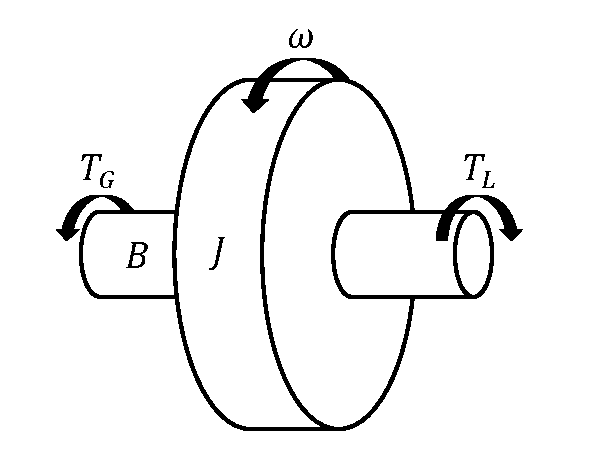
\includegraphics[width=0.4\linewidth]{fig/rotmass.pdf}
	\caption[]{Ideal representation of generators in an \gls{acps} as a rotating mass with inertia and damping.}
	\label{fig:rotmass}
\end{figure}

\begin{figure}[ht!]
	\centering
	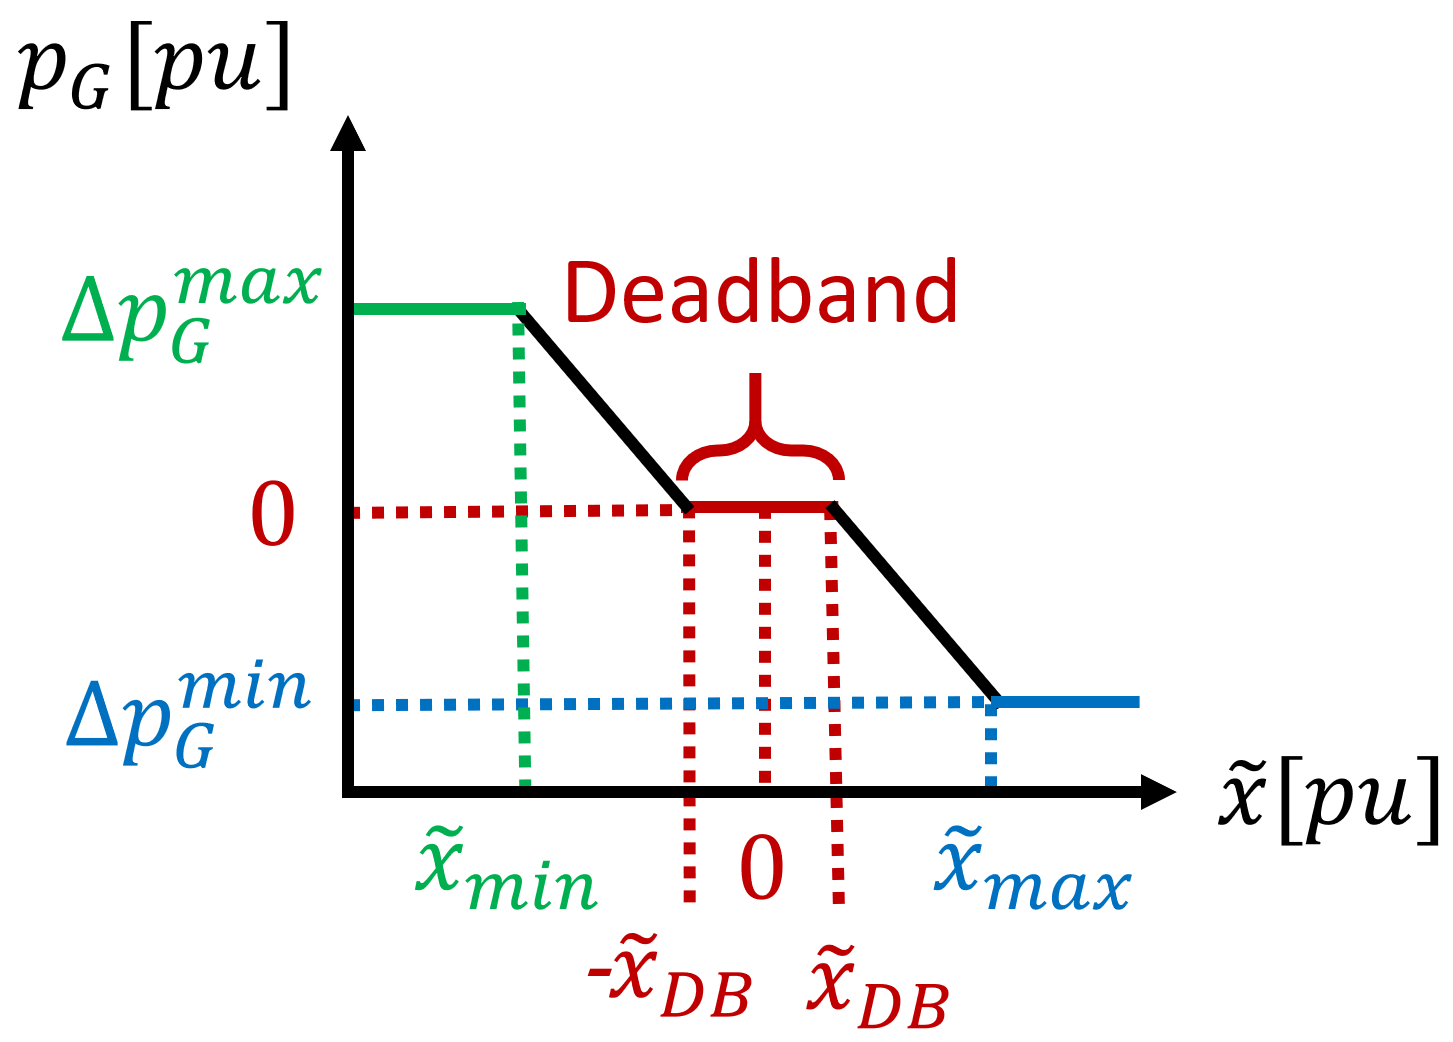
\includegraphics[width=0.4\linewidth]{fig/freqdroop.png}
	\caption[]{Frequency-droop, the main mechanism for primary frequency control.}
	\label{fig:freqdroop}
\end{figure}

\begin{figure}[ht!]
	\centering
	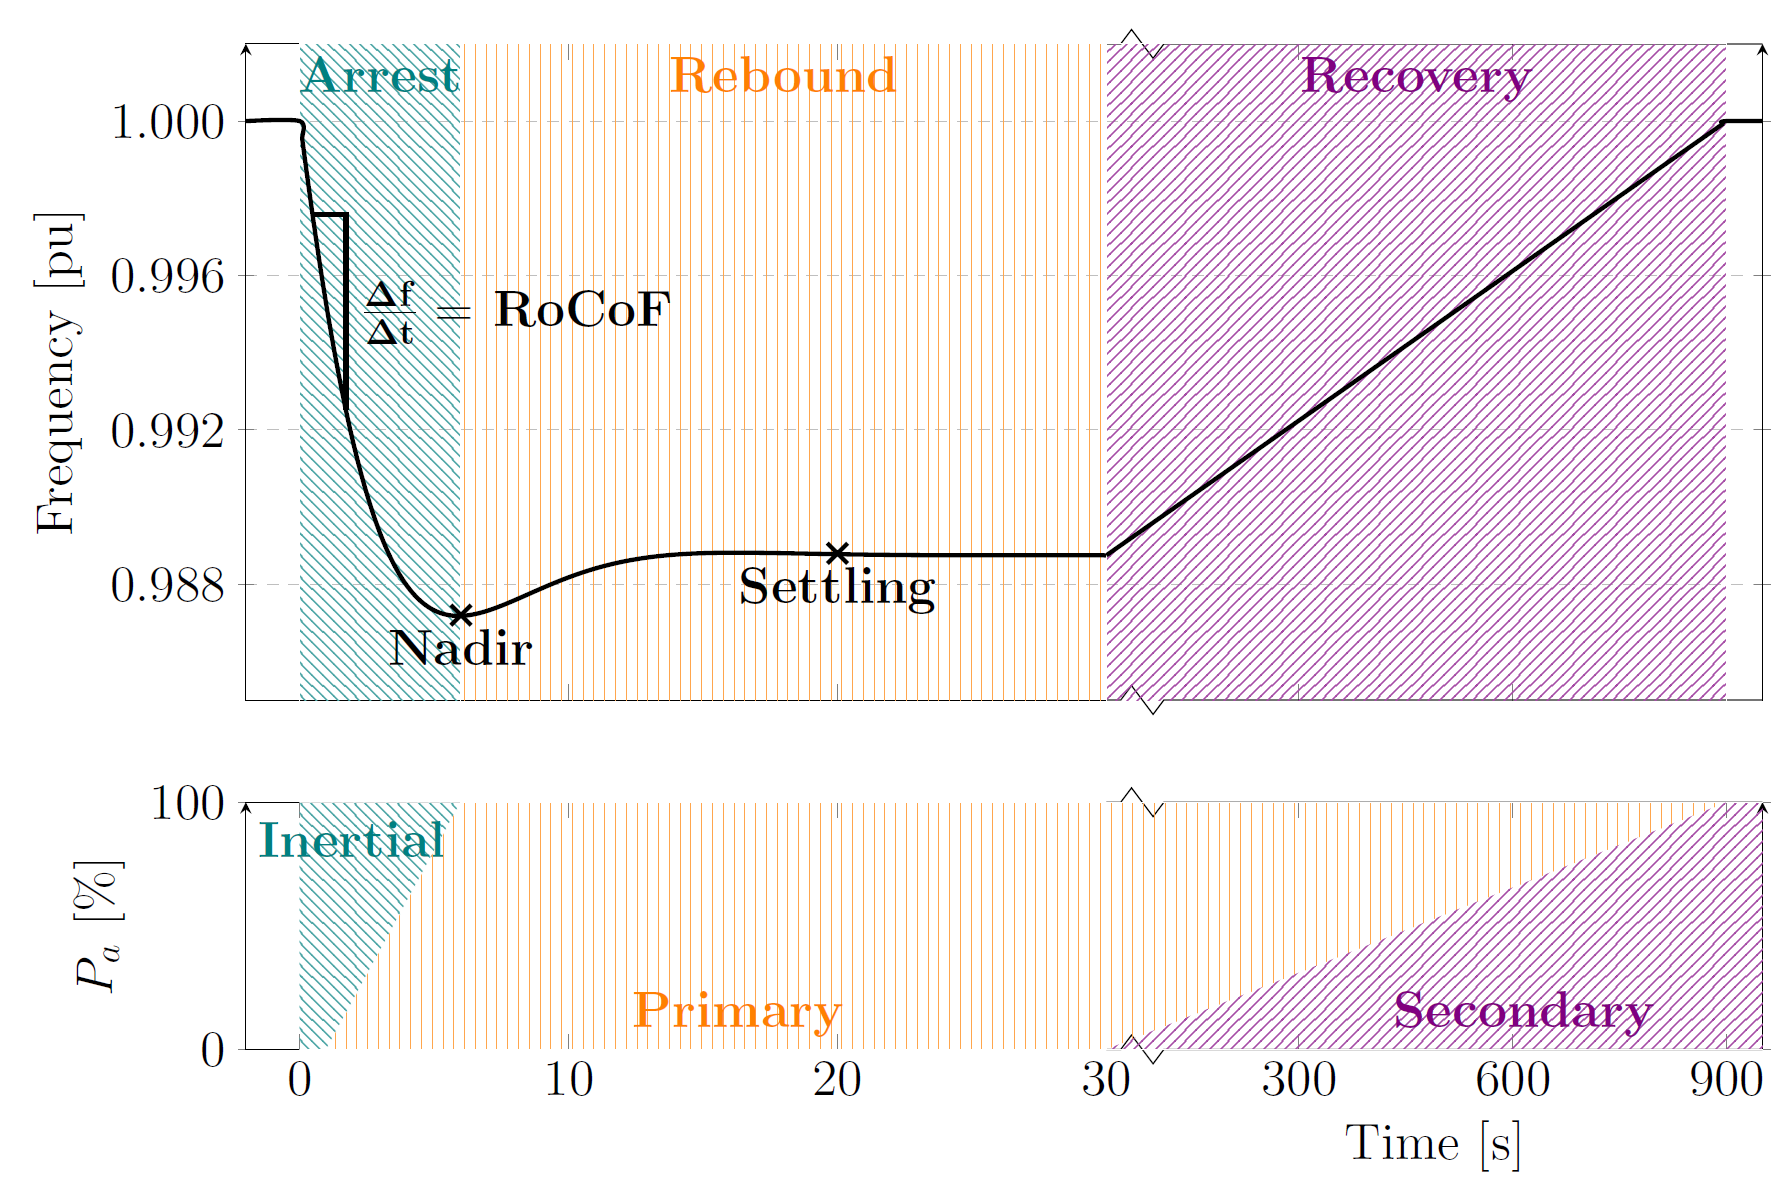
\includegraphics[width=0.6\linewidth]{fig/freqctrl.png}
	\caption[]{The three periods of frequency variation (arresting, rebound and recovery) and the control actions (inertial, primary and secondary) following a perturbation caused by lack of generation.}
	\label{fig:freqctrl}
\end{figure}

\begin{figure}[ht!]
	\centering
	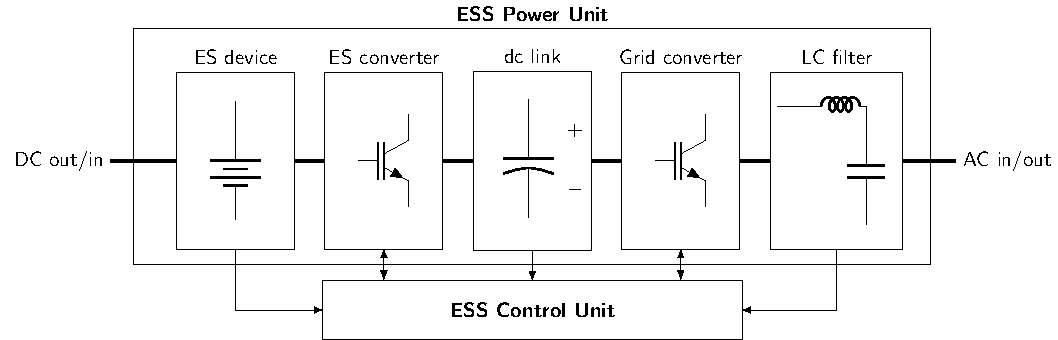
\includegraphics[width=0.8\linewidth]{fig/ess-overview.pdf}
	\caption[]{Elements of a converter-interfaced energy-storage system.}
	\label{fig:ess-overview}
\end{figure}

\begin{figure}[ht!]
	\centering
	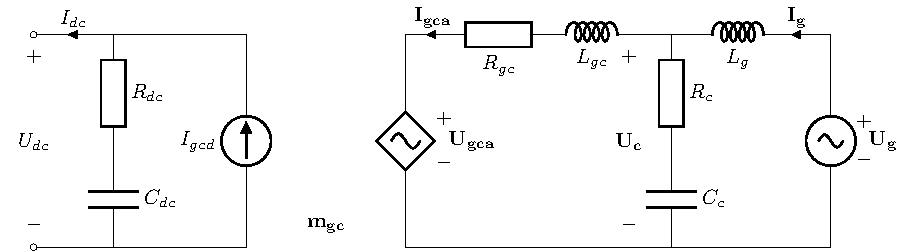
\includegraphics[width=0.8\linewidth]{fig/grid-converter.pdf}
	\caption[]{Schematic representation of the dc link, the grid converter and its LC filter.}
	\label{fig:grid-converter}
\end{figure}

\begin{figure}[ht!]
	\centering
	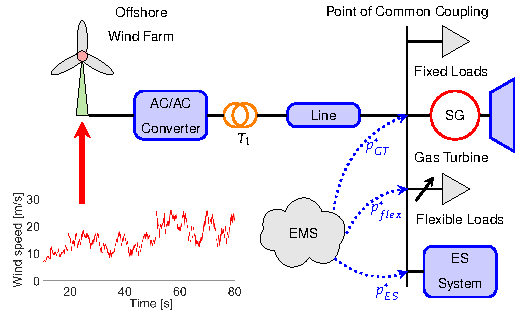
\includegraphics[width=0.8\linewidth]{fig/case-study.pdf}
	\caption[]{Schematic representation of the case study \gls{acps}.}
	\label{fig:case-study}
\end{figure}

%\begin{figure}[h!]
%\begin{center}
%
\includegraphics[width=10cm]{logo1}% This is a *.eps file
%\end{center}
%\caption{ Enter the caption for your figure here.  Repeat as  necessary for each of your figures}\label{fig:1}
%\end{figure}


%\begin{figure}[h!]
%\begin{center}
%
\includegraphics[width=15cm]{logos}
%\end{center}
%\caption{This is a figure with sub figures, \textbf{(A)} is one logo, \textbf{(B)} is a different logo.}\label{fig:2}
%\end{figure}

%%% If you are submitting a figure with subfigures please combine these into one image file with part labels integrated.
%%% If you don't add the figures in the LaTeX files, please upload them when submitting the article.
%%% Frontiers will add the figures at the end of the provisional pdf automatically
%%% The use of LaTeX coding to draw Diagrams/Figures/Structures should be avoided. They should be external callouts including graphics.

\begin{table}[htp!]
\caption{Summary of the \gls{ess} parameters obtained using the proposed procedure.}
\centering
%% \tablesize{} %% You can specify the fontsize here, e.g., \tablesize{\footnotesize}. If commented out \small will be used.
\begin{tabular}{lrl|lrl}
    \toprule
    \textbf{Parameter}	& \textbf{Value} & \textbf{Unit} & \textbf{Parameter}	& \textbf{Value} & \textbf{Unit} \\
    \midrule
	$ P_{es1} $ & 1.62 & \si{\mega\watt} & $ E_{es1} $ & 50.88 & \si{\kilo\watt\hour} \\
	$ U_{dc} $ & 771 & \si{\volt} & $ \Delta U_{dc}^{max}$ & 96 & \si{\volt} \\
	$ T_r $ & 10 & \si{\milli\second} & $ \Delta P_{dc}^{max} $ & 143.9 & \si{\kilo\watt} \\
	$ P_{losses}^{es1} $ & 25 & \si{\kilo\watt} & $ C_{dc} $ & 9.7 & \si{\milli\farad} \\
	$ P_{g} $ & 7.8 & \si{\mega\watt} & $ S_{gc} $ & 9.75 & \si{\mega\volt\ampere} \\ 
	$ U_{2n} $ & 818 & \si{\volt} & $ \Delta I_{gca}$ & 0.15 & pu \\
	$ f_{sw} $ & 4.2 & \si{\kilo\hertz} & $L_{gc}$ & 7.41 & \si{\milli\henry} \\	
    $ L_{g} $ & 10.8 & \si{\milli\henry} & $C_{c}$ & 1.6 & \si{\milli\farad} \\
    $ f_{0} $ & 1.91 & \si{\kilo\hertz} & $R_{c}$ & 15.9 & \si{\milli\ohm} \\
%    \bottomrule
\end{tabular}
\label{tab:results-case-study}
\end{table}


\begin{table}[htbp!]
\caption{Parameters of the \gls{acps} of an offshore oil and gas platform in the Norwegian Continental Shelf and the requirements for its converter-interfaced \gls{ess}.}
\centering
%% \tablesize{} %% You can specify the fontsize here, e.g., \tablesize{\footnotesize}. If commented out \small will be used.
\begin{tabular}{lrl|lrl}
    \toprule
    \textbf{Parameter}	& \textbf{Value} & \textbf{Unit} & \textbf{Parameter}	& \textbf{Value} & \textbf{Unit} \\
    \midrule
	$ S_b $ & 70 & \si{\mega\watt} & $ \omega_s $ & 377 & \si{\radian\per\second} \\
	$ r_{tr} $ & 0.100 & pu & $ r_{ss} $ & 0.025 & pu \\
	$ M_{GT} $ & 5.1 & \si{\second} & $ D_{min} $ & 1.9 & pu \\
	$ D_{flex} $ & 0.87 & pu & $ D_{es} $ & 1.03 & pu \\
	$ P_{ELY} $ & 6 & \si{\mega\watt} & $ P_{FC} $ & 4 & \si{\mega\watt} \\ 
	$(t_b - t_a)$ & 20 & \si{\second} & $(t_c - t_b)$ & 300 & \si{\second}\\
    %\bottomrule
\end{tabular}
\label{tab:par-case-study}
\end{table}

\end{document}
